\subsection{Compressing diagonal slices}\label{sec:compression}

The quadrilateral in Proposition~\ref{prop:quadrilateral} bounds the initial
exponents of sections.  We next reduce its jet tests to those of the triangle
\[
 P_t=\conv\{(-b,0),(a,0),(0,c)\}.
\]
Since $a+b=dH$ and $c=1/d$, this triangle has area
$c(a+b)/2=H/2$.
The reduction preserves the length of each diagonal slice and moves its
lower endpoint to height zero.  Throughout this subsection we test the full
monomial spaces $\mathcal M(kQ_t)$ and $\mathcal M(kP_t)$.  The initial
monomials of sections need only span a subspace of the former.

\begin{lemma}[Diagonal slices]\label{lem:slices}
For $-b\le q\le a$, the slice of $Q_t$ on the line
$\alpha-\beta=q$ has length in the $\beta$ coordinate equal to
\[
 \ell_t(q)=
 \begin{cases}
 c(1+q/b),&-b\le q\le0,\\[2pt]
 c(1-q/a),&0\le q\le a.
 \end{cases}
\]
There are no slices outside this interval, and
\[
 P_t=\{(q,h):-b\le q\le a,\ 0\le h\le\ell_t(q)\}.
\]
\end{lemma}

\begin{proof}
The strict inequality defining $t$ is equivalent to
\[
 c(a+b)>ab.
\]
Thus $(c,c)$ lies strictly beyond the segment joining $(a,0)$ to $(0,b)$,
on the side away from the origin.  In the coordinates
$(q,\beta)=(\alpha-\beta,\beta)$, the four vertices of $Q_t$, in cyclic
order, are
\[
 (0,0),\quad (a,0),\quad (0,c),\quad (-b,b).
\]
For $0\le q\le a$, the slice runs from $\beta=0$ to
$\beta=c(1-q/a)$.  For $-b\le q\le0$, it runs from
\[
 \beta=-q
 \qquad\text{to}\qquad
 \beta=c+\frac{c-b}{b}q.
\]
Subtracting the endpoints gives the stated formula.  The region below
this tent is precisely $P_t$, as illustrated in Figure~\ref{fig:compression}.
\end{proof}

\begin{figure}[tbp]
\centering
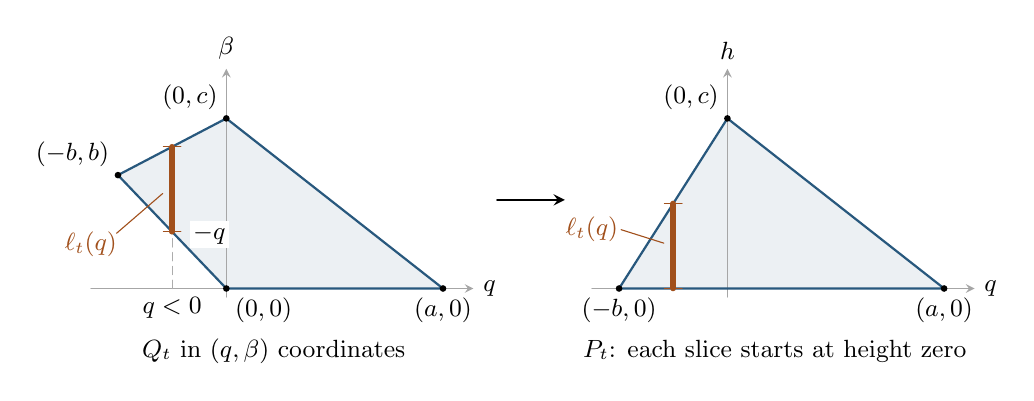
\begin{tikzpicture}[x=.86cm,y=.90cm,font=\small,
  line cap=round,line join=round,>=stealth]
  \definecolor{diagramblue}{RGB}{40,88,125}
  \definecolor{diagramorange}{RGB}{161,80,28}
  \begin{scope}
    \fill[diagramblue!9] (0,0)--(3.2,0)--(0,2.4)--(-1.6,1.6)--cycle;
    \draw[->,gray!70] (-2.0,0)--(3.65,0) node[right,text=black] {$q$};
    \draw[->,gray!70] (0,-.12)--(0,3.1) node[above,text=black] {$\beta$};
    \draw[diagramblue,thick] (0,0)--(3.2,0)--(0,2.4)--(-1.6,1.6)--cycle;
    \draw[densely dashed,gray!65] (-.8,0)--(-.8,.8);
    \draw[diagramorange,line width=2pt] (-.8,.8)--(-.8,2.0);
    \draw[diagramorange] (-.93,.8)--(-.67,.8) (-.93,2.0)--(-.67,2.0);
    \node[diagramorange] at (-2.0,.62) {$\ell_t(q)$};
    \draw[diagramorange,thin] (-1.62,.78)--(-.94,1.34);
    \node[anchor=west,fill=white,inner sep=1.3pt] at (-.55,.76) {$-q$};
    \fill (0,0) circle (1.2pt) (3.2,0) circle (1.2pt)
          (0,2.4) circle (1.2pt) (-1.6,1.6) circle (1.2pt);
    \node[below right,inner sep=3pt] at (0,0) {$(0,0)$};
    \node[below,inner sep=3pt] at (3.2,0) {$(a,0)$};
    \node[above left,inner sep=3pt] at (0,2.4) {$(0,c)$};
    \node[above left,inner sep=3pt] at (-1.6,1.6) {$(-b,b)$};
    \node[below,inner sep=3pt] at (-.8,0) {$q<0$};
    \node[align=center] at (.7,-.88) {$Q_t$ in $(q,\beta)$ coordinates};
  \end{scope}
  \draw[->,thick] (4.0,1.25)--(5.0,1.25);
  \begin{scope}[shift={(7.4,0)}]
    \fill[diagramblue!9] (-1.6,0)--(3.2,0)--(0,2.4)--cycle;
    \draw[->,gray!70] (-2.0,0)--(3.65,0) node[right,text=black] {$q$};
    \draw[->,gray!70] (0,-.12)--(0,3.1) node[above,text=black] {$h$};
    \draw[diagramblue,thick] (-1.6,0)--(3.2,0)--(0,2.4)--cycle;
    \draw[diagramorange,line width=2pt] (-.8,0)--(-.8,1.2);
    \draw[diagramorange] (-.93,0)--(-.67,0) (-.93,1.2)--(-.67,1.2);
    \node[diagramorange] at (-2.0,.83) {$\ell_t(q)$};
    \draw[diagramorange,thin] (-1.57,.83)--(-.94,.64);
    \fill (-1.6,0) circle (1.2pt) (3.2,0) circle (1.2pt)
          (0,2.4) circle (1.2pt);
    \node[below,inner sep=3pt] at (-1.6,0) {$(-b,0)$};
    \node[below,inner sep=3pt] at (3.2,0) {$(a,0)$};
    \node[above left,inner sep=3pt] at (0,2.4) {$(0,c)$};
    \node[align=center] at (.7,-.88) {$P_t$: each slice starts at height zero};
  \end{scope}
\end{tikzpicture}
\caption{Diagonal compression of exponent slices. For $c(a+b)>ab$, the
change $q=\alpha-\beta$ turns $Q_t$ into the quadrilateral on the left.
Moving each vertical slice down to height zero gives $P_t$, with the
same slice length $\ell_t(q)$. The highlighted slice has $q<0$ and lower
endpoint $-q$. This diagram describes the containing regions; the jet
transfer is proved by convergence of finite jet matrices.}
\label{fig:compression}
\end{figure}



\begin{proposition}[Diagonal compression]\label{prop:compression}
Let $k,m,r$ be positive integers.  If $\mathcal M(kP_t)$ has injective
order-$m$ jets at some $r$ distinct points of $\T$, then
$\mathcal M(kQ_t)$ has injective order-$m$ jets at some $r$ distinct
points of $\T$.
\end{proposition}

\begin{proof}
Use the torus coordinates
\[
 (x,z)=(u,v/u),\qquad (u,v)=(x,xz).
\]
A monomial $x^\alpha z^\beta$ becomes $u^qv^\beta$, where
$q=\alpha-\beta$.  For every nonempty integer slice $q$ of $kQ_t$, write
\[
 \beta_q^-=
 \min\{\beta\in\Z:(q+\beta,\beta)\in kQ_t\},
 \qquad
 \beta_q^+=
 \max\{\beta\in\Z:(q+\beta,\beta)\in kQ_t\}.
\]
Convexity of the slice implies that all integers between these endpoints
occur.  Hence the slice has the basis
\begin{equation}\label{eq:compression-row-basis}
 u^qv^{\beta_q^-}(v-1)^h,
 \qquad 0\le h\le\beta_q^+-\beta_q^-.
\end{equation}
Indeed, expanding $(v-1)^h$ gives a triangular change of basis from the
consecutive powers of $v$, with diagonal entries equal to one.  By Lemma~\ref{lem:slices},
\[
 h\le\beta_q^+-\beta_q^-
 \le k\ell_t(q/k).
\]
Consequently every pair $(q,h)$ in
\eqref{eq:compression-row-basis} belongs to $kP_t\cap\Z^2$.
These pairs are distinct, both within each slice and between different slices.

Let $(u_i,y_i)$, $1\le i\le r$, be distinct torus points giving an
injective jet test for $\mathcal M(kP_t)$, now written in the variables
$(u,y)$.  For a positive parameter $s$, substitute $v=1+sy$ into
\eqref{eq:compression-row-basis} and divide its member indexed by $h$
by $s^h$.  The resulting functions are
\begin{equation}\label{eq:compression-limit}
 u^q(1+sy)^{\beta_q^-}y^h
 \longrightarrow u^qy^h
 \qquad (s\longrightarrow0^+).
\end{equation}
The convergence is locally uniform, with every spatial derivative, on
fixed neighborhoods of the finitely many test points.  To see this,
choose bounded neighborhoods on which $u$ stays away from zero and
then take $s$ small enough that $|sy|<1/2$ there.  The factors
$(1+sy)^{\beta_q^-}$ are holomorphic and converge uniformly to one on
slightly larger neighborhoods, so the derivative assertion follows
from the Cauchy estimates.  The argument also applies to negative
Laurent powers, since $1+sy$ stays away from zero.

The distinct limiting monomials in \eqref{eq:compression-limit} span
a subspace of $\mathcal M(kP_t)$, so their jet matrix has full column
rank.  Lemma~\ref{lem:rank-persistence} gives the same conclusion for
the functions on the left for every sufficiently small positive $s$.
These functions form a rescaled pullback of a basis of
$\mathcal M(kQ_t)$.

For such an $s$, the corresponding points in the original torus are
\[
 \left(u_i,\frac{1+sy_i}{u_i}\right),\qquad 1\le i\le r.
\]
They lie in $\T$ because $u_i\ne0$ and $1+sy_i\ne0$.  They are distinct:
equality of two images forces equality first of their $u$ coordinates
and then of their $y$ coordinates.  The coordinate map
\[
 (u,y)\longmapsto\left(u,\frac{1+sy}{u}\right)
\]
has Jacobian determinant $s/u\ne0$, and therefore preserves orders of
vanishing at these points.  The full-column-rank conclusion is thus
exactly the required injectivity for $\mathcal M(kQ_t)$.
\end{proof}

The two transfers now give the test needed on the surface.

\begin{corollary}[From the triangle to the surface]
\label{cor:surface-transfer}
Let $k,m,r$ be positive integers.  If $\mathcal M(kP_t)$ has injective
order-$m$ jets at some $r$ distinct torus points, then $H^0(S,kL)$ has
injective order-$m$ jets at some $r$ distinct points of $S$.
\end{corollary}

\begin{proof}
If $H^0(S,kL)=0$, the conclusion is immediate.  Otherwise,
Proposition~\ref{prop:compression} gives such a jet test for
$\mathcal M(kQ_t)$.  Trivialize $L$ in the fixed coordinate chart at
the node and regard the sections of $kL$ as holomorphic germs there.
This identification is injective: a global section vanishing on a
nonempty open subset of the integral surface vanishes identically.
Proposition~\ref{prop:quadrilateral} gives a basis whose distinct
initial monomials lie in $kQ_t$.  Their span therefore has injective
jets at the torus tuple just constructed.  Applying
Proposition~\ref{prop:initial-transfer} gives injective jets for the
section germs at distinct points in the chart, and hence for
$H^0(S,kL)$ on $S$.
\end{proof}
